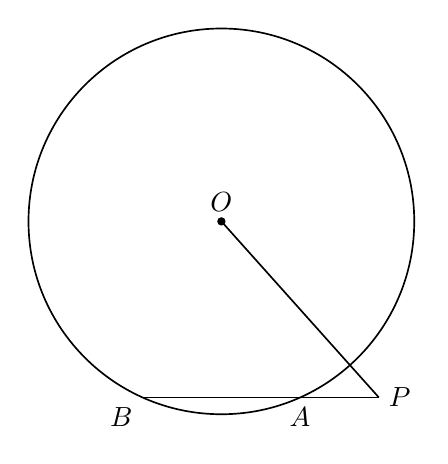
\begin{tikzpicture}[x=1cm,y=1cm,line width=.6pt,font=\normalsize]
\coordinate (O) at (0,0);
\coordinate (A) at (1,-2.2361);
\coordinate (B) at (-1,-2.2361);
\coordinate (P) at (2,-2.2361);
\draw (O) circle[radius=2.4495cm];
\draw (O)--(P);
\draw (B)--(P);
\fill (O) circle (1.5pt);
\node[above] at (O) {$O$};
\node[below] at (A) {$A$};
\node[below left] at (B) {$B$};
\node[right] at (P) {$P$};
\end{tikzpicture}
